%-----------------------------------------------------------Header Starts--------------------------------------

\documentclass[main.tex]{subfiles}

%-----------------------------------------------------------Header Ends--------------------------------------


\graphicspath{ {./image_intro/} }



\begin{document}

\chapter{Introduction}

\pagenumbering{arabic}

\thispagestyle{empty}

\pagestyle{fancy}
\fancyhf{}

\rhead{Page \thepage}
\lhead{\chaptername \ \thechapter}
%\cfoot{Page \thepage}

\section{Background of the research}
Modern technology stands on the shoulder of semiconductor materials for their immensely useful adaptabilities of physical properties specially the electrical conductivity with an applied electrical field. Despite of having superior conductivity, metals have been outcast by the uniqueness of semiconductor materials in controlling the flow of current. For example, in order to perform a logic function, the ability to distinguish between one and zero is necessary. Semiconductor materials have the capability to transform from insulating to conducting with the help of very small amount of voltage known as gate voltage. When the gate voltage is above a certain level, current flows through a small channel between source and drain; making the material conductive. Again, this flow of current is interrupted when gate voltage is below the level. This directional flow of current in semiconductor is basically driven by very dilute concentration of dopants into a host semiconductor (i.e. 10$^{13}$ to 10$^{18}$ dopant atoms/cm$^{3}$ in Si as host material which contains 5$ \times $10$^{22}$ atoms/cm$^{3}$). By inducing such excess or shortage of electrons via doping, variable electrical resistance can be achieved which makes semiconductor materials useful for switching, amplification or energy conversion applications. This class of semiconductor is known as Transistor and they led the most important paradigm shift in technology by miniturization of devices which in turns reduces the energy utilization by thousand folds. The placement of these transistors on the integrated circuit (IC) is important because the more miniaturized dense IC could be made, the less heat loss would happen which eventually will raise the speed of information process. In 1965, Gordon Moore, one of the cofounder of Intel, predicted that the number of transistors placed on an IC will double in every two years. Companies like Intel, Samsung and NVidia are now fabricating transistors less than 20 nm in size at mass scale and NVidia’s new graphics card GF100 is an example of how dense miniaturized a device can become which contains more than 3 Billion transistors. But, this miniaturization to speed up the information process has now reached its saturation limit since it is almost at the edge of atomic scale. On the other side, we are producing more than 2.5 quintillion bytes of data everyday according to Forbes. With days passing by, we are becoming fonder of online based social and financial activities. The energy required for processing this large amount of data is causing global warming at an increased alarming rate. As, the miniaturization of device can no longer provide benefits to us in energy conservation via faster communication, we now must have to think otherwise. \\


In electronics, only the charge of the electron is utilized while it’s another degree of freedom “Spin” remains less remembered. If the spin states can be incorporated with electronic charge to store and process information, the communication will increase by many folds which has been a fascination for decades. Spintronics, an acronym for SPIN TRansport electrONICS, is one of such promising areas which brought us the novel concept of utilizing both the charge and spin of the electrons. Apart from the formerly known classical states of electron's spinning i.e. rotating clockwise or anticlockwise, there are infinite number of spin states that an electron can possess according to quantum mechanics. If these spin states could be controlled like the current flow in transistor, we would have more options beside the conventional switching technique i.e. current off(0) or on(1). That being said, the electrons carry the spin state must be non-volatile as well as spin polarized and the ferromagnetism needs to be capable of gating.  For example, Kreutz \textit{et al.} showed that an organic monolayer, deposited on surface, can provide electrons to compensate the hole carriers of GaMnAs which restrain the ferromagnetism (\(T_C < 170 K\)) \cite{kreutz2003modification}. The control over ferromagnetism by changing carrier concentration like Kreutz's research is what we want to achieve at room temperature. \\

Initially, spin injection attempts were limited to the heterostructure comprising a metallic ferromagnet on semiconductor device \cite{Datta1990,DasSarma2000}. But due to serious deficiency of spin injection at metal-semiconductor interface, this idea was replaced by a quest for the ferromagnetism in semiconductor. The concept of ferromagnetic semiconductor was initiated by introducing dilute concentration of magnetic dopants (Mn$^{2+}$) into a semiconductor material, \(Ga_{(1-x)}Mn_xAs \ (x=0.015–0.071)\) \cite{matsukura1998transport}. The ferromagnetism observed in such non-magnetic semiconductors are supposed to be carrier mediated. The excess electrons provided by the dopants delocalize near the fermi level. For certain cases, these delocalized impurity bands become spin polarized and tend to show half-metallic behavior. The materials showed such property were started to be termed as “Dilute Magnetic Semiconductor (DMS)”. In an ideal DMS, the charge carriers are spin polarized and behave like half-metallic which enable the charge carriers to be transported by inducing very small applied electrical or magnetic field. By showing high promises of carrier mediated spin-charge transport, DMS materials have raised a lot of enthusiasm in scientific community in the recent years to extend the established CMOS (Complementary Metal Oxide Semiconductor) based electronics towards spintronics devices. \\

\section{Dilute Magnetic Semiconductors (DMS)}

Dilute magnetic semiconductors are actually non – magnetic materials containing very small amounts of magnetic ions as dopants. Due to these magnetic dopants, the non – magnetic materials show dilute ferromagnetism. But the basic difference between DMS and other ferromagnetic materials is DMS’s half metallic behavior which alone controls the spin-charge transport in these materials. Hence, it is noteworthy to revisit the concept of spin polarization and half metallic behavior before going further about DMS. \\

Spin polarization can be expressed as the ratio of the density of states of up-spin and down-spin electrons at fermi level. The degree of polarization is \( P=\frac{N_{up}-N_{down}}{N_{up}+N_{down}} \) where up-spin ($N_{up}$) and down-spin ($N_{down}$) electrons denote the electrons polarized in opposite directions. In paramagnetic materials, the degree of polarization is 0 and in conventional ferromagnetic materials the value is between 0 and 1. Only for the cases of half-metal, the degree of polarization is 1. The schematic density of states of an ideal half metal is given in Fig 1(g). In an ideal half-metal, for specific polarized electrons (either $N_{up}$ or $N_{down}$) will have density of states in fermi level which does not have any gap between conduction and valence band. For other set of polarized electrons, there will be no density of states in fermi level just like an intrinsic semiconductor. This means that all electrons at fermi level in half-metal are completely polarized and for the presence of gapless density of states at fermi level, the polarized electrons will behave like free electrons of metal. For this reason, these materials are called as half-metal. The concept of half-metal was first predicted by Groot \textit{et al.} during the electronic band structure calculation of NiMnSb and PtMnSb \cite{groot1983}. Coey \textit{et al.} explained the half metallic behavior in Cr$O_2$ and predicted that the half-metallicity in semiconductors can be classified in two types as showed in Fig 1 (h) $\&$ (i) \cite{coey2002half}. 

\begin{figure}[!htb]
\centering
	\begin{subfigure}[h]{0.32\textwidth}
		\centering
		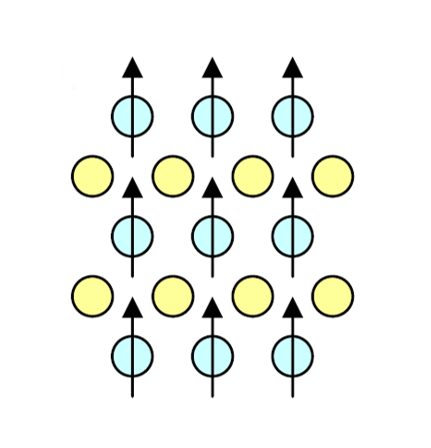
\includegraphics[width=\linewidth]{dms1}
  		\caption{Magnetic material}
   		\label{fig:sub-first}
	\end{subfigure}
	%\hfill
	\begin{subfigure}[h]{0.32\textwidth}
  		\centering
  		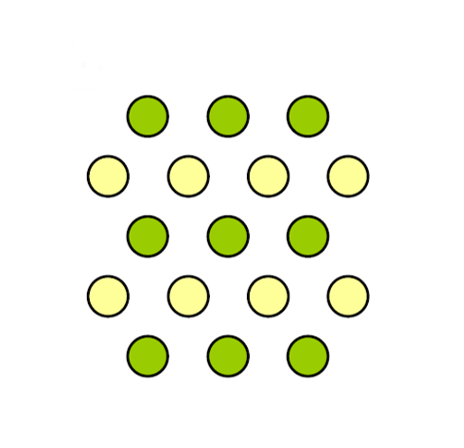
\includegraphics[width=\linewidth]{dms2}
  		\caption{Non-magnetic material}
  		\label{fig:sub-second}
	\end{subfigure}
	\begin{subfigure}[h]{0.32\textwidth}
  		\centering
  		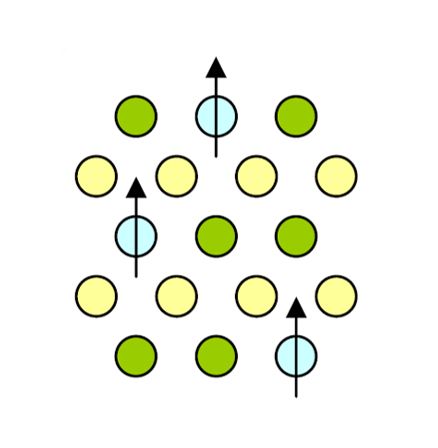
\includegraphics[width=\linewidth]{dms3}
  		\caption{Dilute magnetic semiconductor}
  		\label{fig:sub-second}
	\end{subfigure}
	\begin{subfigure}[h]{0.32\textwidth}
  		\centering
  		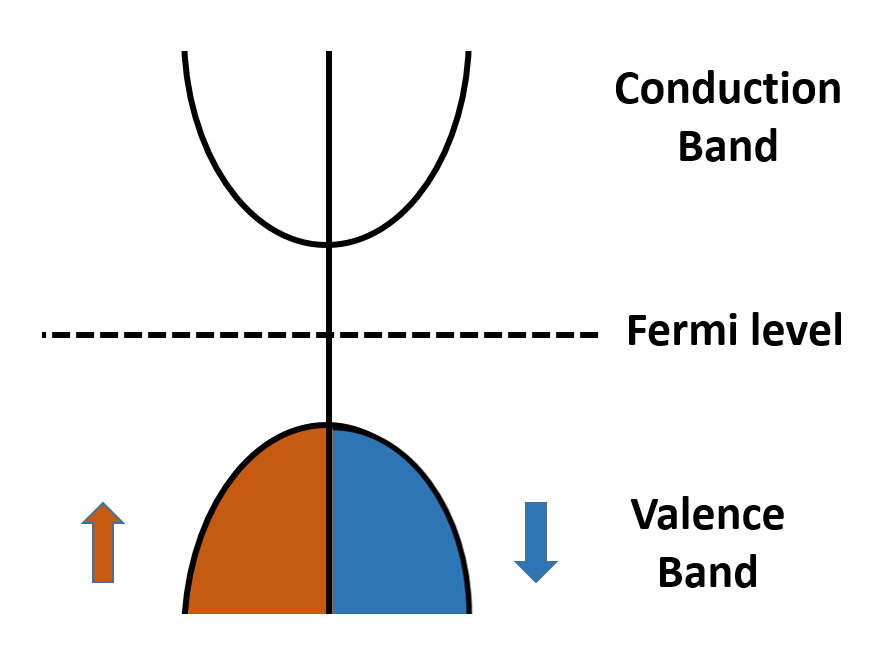
\includegraphics[width=\linewidth]{dos_intrinsic_semiconductor}
  		\caption{Intrinsic semiconductor}
  		\label{fig:sub-second}
	\end{subfigure}
	\begin{subfigure}[h]{0.32\textwidth}
  		\centering
  		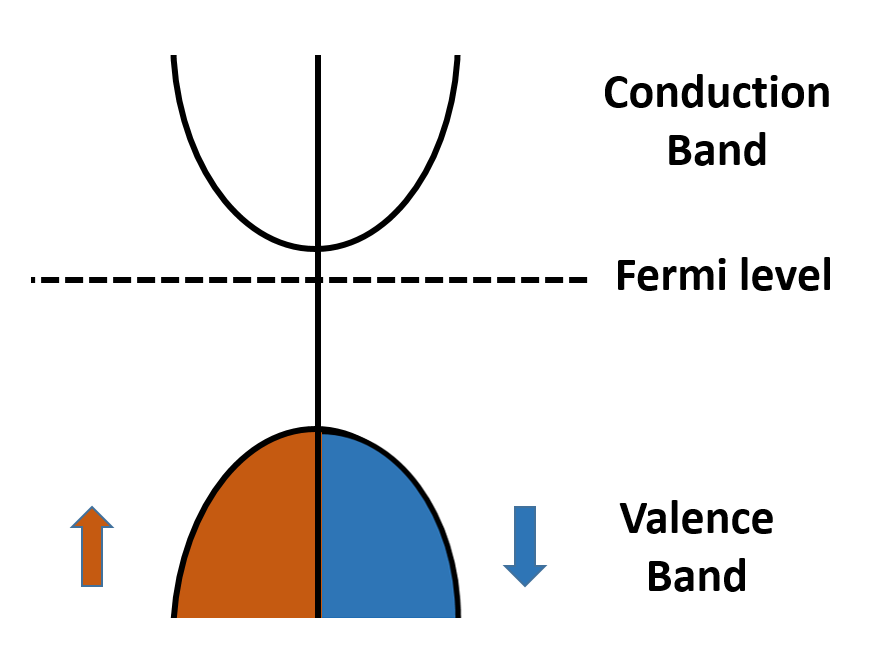
\includegraphics[width=\linewidth]{dos_ntype_semiconductor}
  		\caption{n type semiconductor}
  		\label{fig:sub-second}
	\end{subfigure}
	\begin{subfigure}[h]{0.32\textwidth}
  		\centering
  		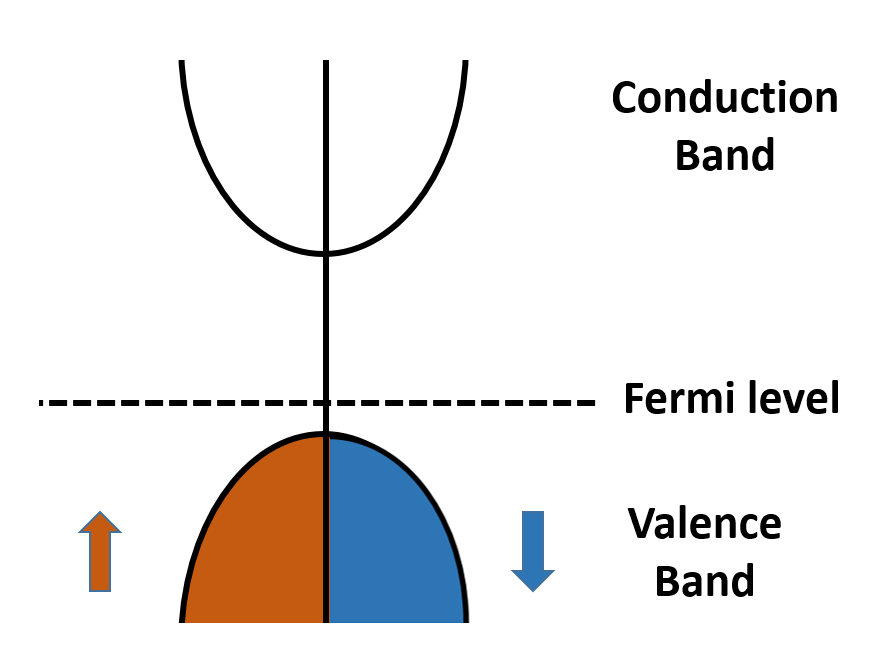
\includegraphics[width=\linewidth]{dos_ptype_semiconductor}
  		\caption{p type semiconductor}
  		\label{fig:sub-second}
	\end{subfigure}
	\begin{subfigure}[h]{0.32\textwidth}
  		\centering
  		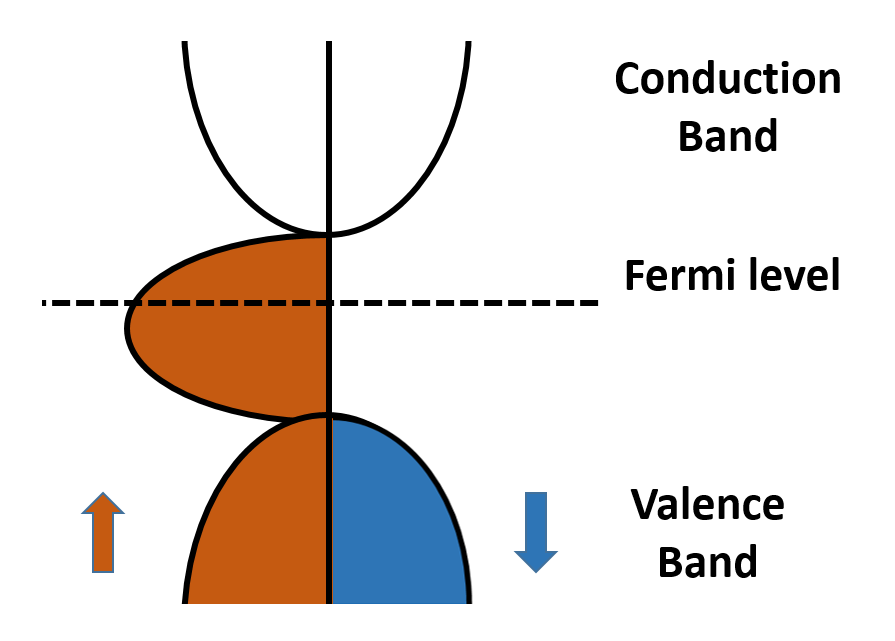
\includegraphics[width=\linewidth]{dos_half_metal}
  		\caption{Ideal half metal}
  		\label{fig:sub-second}
	\end{subfigure}
	\begin{subfigure}[h]{0.32\textwidth}
  		\centering
  		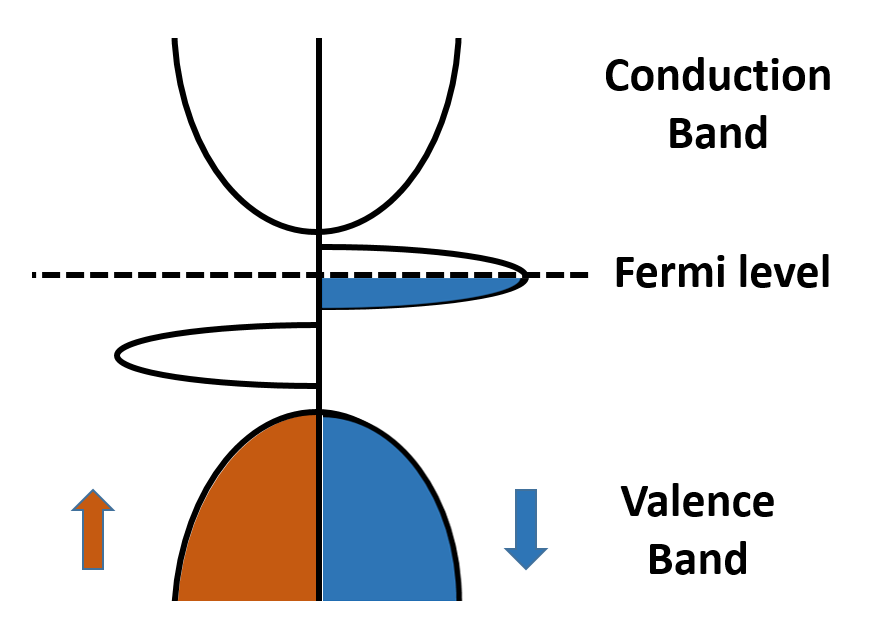
\includegraphics[width=\linewidth]{dos_half_metallic1}
  		\caption{Type-I half metallic semiconductor}
  		\label{fig:sub-second}
	\end{subfigure}
	\begin{subfigure}[h]{0.32\textwidth}
  		\centering
  		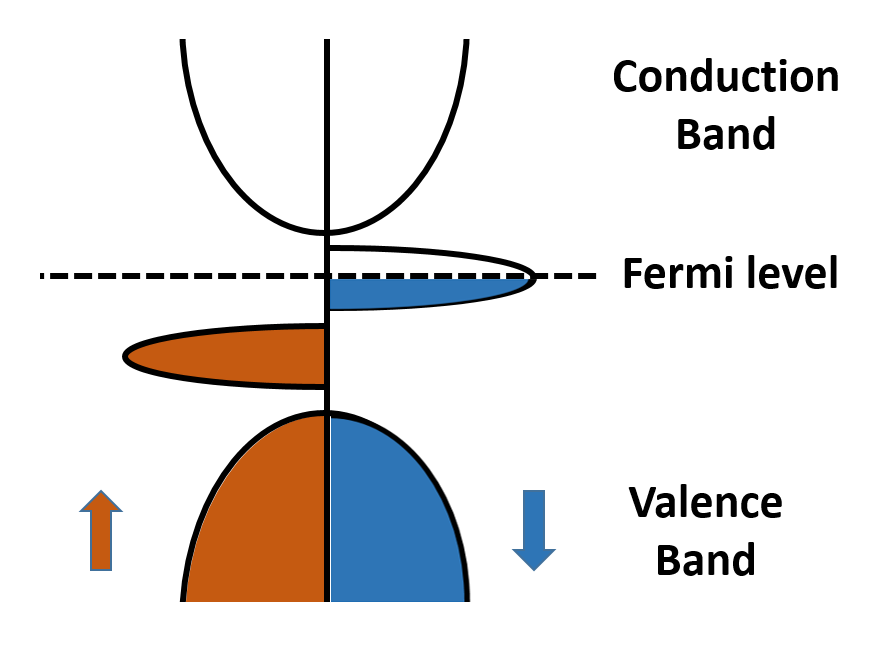
\includegraphics[width=\linewidth]{dos_half_metallic2}
  		\caption{Type-II half metallic semiconductor}
  		\label{fig:sub-second}
	\end{subfigure}
\caption{(a-c) Difference between ferromagnetic material, non-ferromagnetic material and dilute magnetic semiconductor. (d-i) Density of states of different types of semiconductor, ideal half metal and half-metallic semiconductors}
\label{fig:TEM_PT}

\end{figure}
\FloatBarrier

The bands at fermi level are originated from the delocalized d or f orbital electrons in both types of half-metallic semiconductors. From Fig 1 (h) $\&$ (i), it can be clearly understood that the bands in type I material are comprised of less than half filled d or f orbital electrons while in type II, the bands are comprised of more than half-filled d or f orbital electrons. Although the density of states of half-metallic semiconductor deviate from the gapless states of half-metals, the spin polarized delocalized electrons can be transported by hopping from one site to another \cite{coey2002half}. \\ 

In dilute magnetic semiconductor, the magnetic dopants have excess electrons which delocalize at fermi level. It is noteworthy to mention that the dilute magnetic semiconductors should have non-zero spin polarization to achieve half-metallicity. If the half-metallic behavior can be made stable at room temperature, only then the DMS materials will be able to bring a paradigm shift in technology by integrated in logic devices, spin polarized light emitting diodes, non – volatile memory storages, spin field effect transistors etc. 

\section{Current challenges in DMS research}

The earliest discovery of dilute magnetic semiconductors were reported for Mn doped II-IV and III-V alloys. In 1988, Furdyna \textit{et al.} studied the physical properties of $Cd_{(1-x)}Mn_{x}Se$ and $Hg_{(1-x)}Mn_{x}Te$ but the curie temperature was around 40 K \cite{furdyna1988diluted}. In 1989, Munekata \textit{et al.} observed the properties of dilute magnetic semiconductor in $Ga_{(1-x)}Mn_{x}As$ while the curie temperature was around 100 K \cite{munekata1989diluted}. Since then half metallic behavior in these materials specially in $Ga_{(1-x)}Mn_{x}As$ was deliberately studied but the curie temperature could not be raised above 170 K. The quest for a room temperature DMS got a new dimension when Matsumoto \textit{et al.} reported extrinsic ferromagnetism in $Ti_{(1-x)}Co_{x}O_{2}$ which has very high curie temperature (600 K) \cite{matsumoto2001room}. To this day, dilute ferromagnetism at room temperature has been observed in non-magnetic oxides like ZnO, $In_{2}O_{3}$, $CeO_{2}$, $SnO_{2}$, $CuO_{2}$ etc \cite{yi2010ferromagnetism, ueda2001magnetic, ogale2003high, philip2004high}. But the concept of making DMS by doping of magnetic impurities was changed when room temperature ferromagnetism was observed in undoped non-magnetic oxides. Besides, magnetic clusters and secondary phases have been found to contribute to extrinsic ferromagnetism in these oxides \cite{sundaresan2006ferromagnetism, hong2006room, venkatesan2004thin}. Therefore, creation of any spintronics device based on these oxide based DMS materials remains halted due to the true understanding of the origin of ferromagnetism in these materials. 

\section{Objective of this research}

The aim of this research is focused on the dilute ferromagnetism in $Ti_{(1-x)}Sm_{x}O_{2}$ (0 $\leq x \leq$ 0.2) nanoparticles. Among the wide bandgap semiconductors, Ti$O_{2}$ is the most extensively studied material for its superior chemical stability and high curie temperature. The primary reason for $Sm^{3+}$ substitution in Ti$O_{2}$ is to create oxygen vacancy. The electronic configuration of Sm and Ti are [Xe] $4f^{6}$ $6s^{2}$ and [Ar] $3d^{2}$ $4s^{2}$ respectively. But the preference of $Sm^{3+}$ ($Sm^{3+}$=[Xe] $4f^{5}$) substitution stems from the fact that it has odd number of excess electrons when it substitutes $Ti^{4+}$ in Ti$O_{2}$. The number of excess electrons is important because they are supposed to be delocalized and induced non-zero spin polarization at fermi level. The delocalized electrons tend to pair themselves by crystal field splitting for energy minimization. For example, $Fe^{2+}$ ([Ar] $3d^{6}$) has four unpaired d oribital electrons but after crystal field splitting $Fe^{2+}$ tends to have 3 pairs of d electrons which in turns yield near to zero spin polarization. On another case, $Fe^{3+}$ ([Ar] $3d^{5}$) five unpaired electrons in valence band. Because having odd number of electrons, it is impossible to nullify the net spin polarization of $Fe^{3+}$ by electron's ownselves pairing mechanism. However, in this research $Sm^{3+}$ was chosen for its odd numbers of f orbital electrons in valence band which are supposed to exhibit strong spin-orbit interaction. \\

Another reason of $Sm^{3+}$ substitution in Ti$O_{2}$ is its larger ionic radius ($Sm^{3+}$=1.08 $\AA$ and $Ti^{4+}$=0.68 $\AA$). One of the main goals of this research is to investigate what happens beyond the solid solubility limit of $Sm^{3+}$ substitution. As it is previously stated that there are discrepancies on the origin of ferromagnetism in oxide DMS materials which mostly revolve around the nature of substitution. Hence it is crucial to investigate the structural purity beyond solid solubility limit of substitution such as the formation $\&$ growth of the interface of any 2nd phase and their effect on optical and magnetic properties. So, the aim of this research can be summarized as:

\begin{itemize}
  \item To study the effect of $Sm^{3+}$ substitution on the structural, optical and magnetic properties of Ti$O_{2}$
  \item To investigate the nature of formation and growth of any second phase beyond solid solubility limit of substitution
\end{itemize}

\section{Thesis overview}

Chapter 2 starts with a brief review on recent progress in dilute magnetic semiconductors and the experimental techniques to investigate the spin polarization in these materials. It will also discuss several theoretical models on the origin of ferromagnetism in DMS. Finally there will be a brief review on recent theoretical and experimental research on Ti$O_{2}$. Chapter 3 describes the experimental methodology and introduces the detailed synthesis process followed by the structural, morphology, optical and magnetic characterization techniques. Chapter 4 discusses the results obtained from experiments and how they support an elucidation of this research which is concisely given in Chapter 5.      

\thispagestyle{fancy}


\end{document}







